\begin{tcolorbox}
Die Produktfunktionen beschreiben jede einzelne Funktion des Produkts mittels Anwendungsfalldiagrammen und Anwendungsfalltabellen.
Diese sollen möglichst ausschlaggebend für das zu entwickelnde System sein und nicht simple Produktfunktionen wie z.B. Login, Account erstellen, Gruppe beitreten, Passwort ändern oder ähnliches zeigen.
\autoref{fig:anwendungsfall-app-tabelle-xx-1} stellt eine exemplarische Tabelle für die Beschreibung eines Anwendungsfalls dar. Stil und Formatierung sind variabel. Nicht jede Zelle muss immer gefüllt sein.
\\\\
In  Tabelle~\autoref{fig:akteur-tabelle} werden alle auftretenden Akteure beschrieben.


\end{tcolorbox}

\begin{figure}[h]
	\centering
	
	\begin{tabularx}{\textwidth}{ p{.2\textwidth} | p{.2\textwidth} | X }
		\textbf{Akteur} & \textbf{Beschreibung} & \textbf{Verwendet in Anwendungsfall} \\ \hline
		Informatiker & Programmiert tolle Sachen & Programmieren, Kaffee trinken, Schlafen
	\end{tabularx}
	
	\caption{Beschreibung der Akteure}
	\label{fig:akteur-tabelle}
\end{figure}

%%%%%%%%%%%%%%%
%% Eigene Arbeit %%
%%%%%%%%%%%%%%%

%%%%%%%%%%%%%%%
%% Anwendungsfall 1 %%
%%%%%%%%%%%%%%%

\section{Anwendungsfalldiagramm}

\begin{figure}[h]

	\hspace{-5cm}
	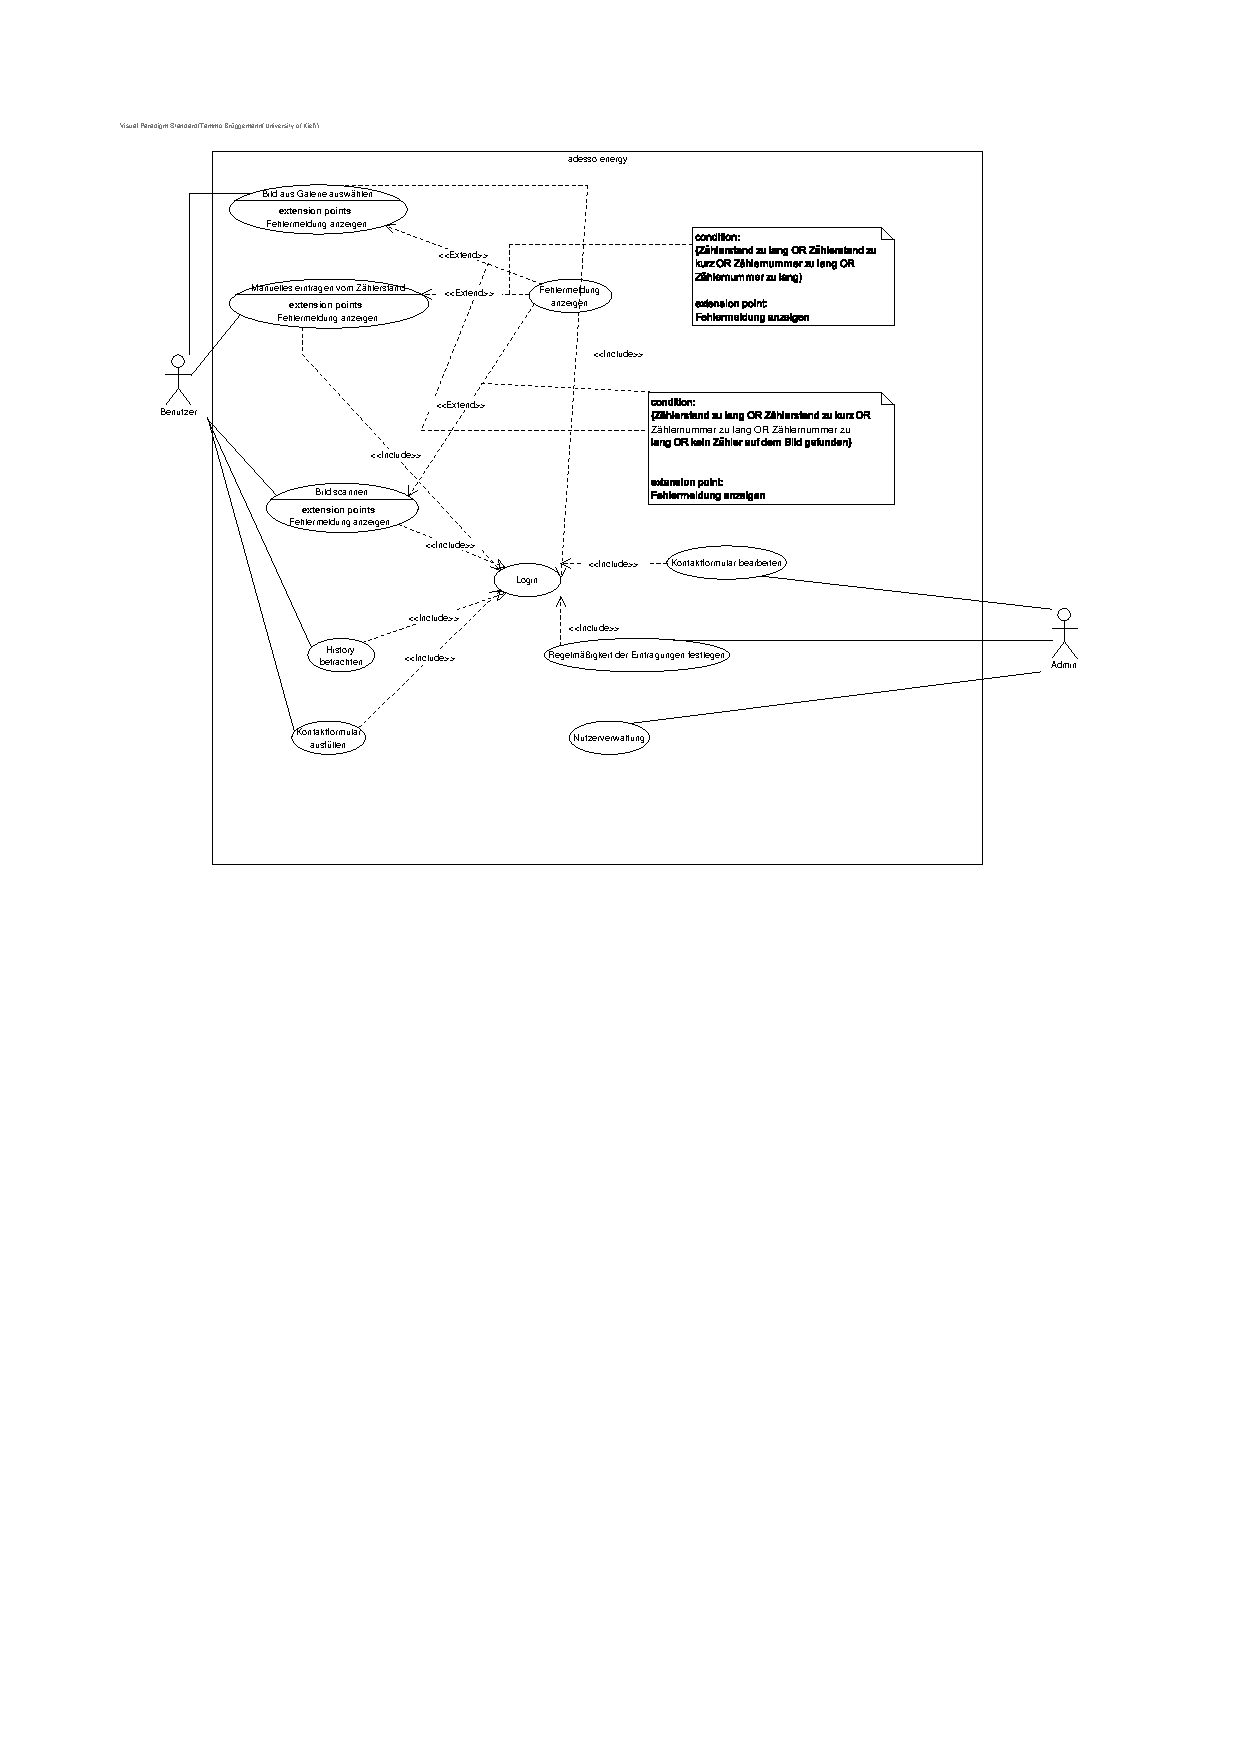
\includegraphics[width=25 cm, height = 45cm]{./img/mustCase}
%	\centering
%	\missingfigure{Anwendungsfalldiagramm - App}		
%	\caption{Anwendungsfalldiagramm - App}
%	\label{fig:anwendungsfalldiagramm-app}
\end{figure}

\newpage

\begin{figure}[h]
	\centering
	\begin{tabularx}{\textwidth}{ X | X }
		\textbf{Anwendungsfall ID} & M1 \\ \hline
		\textbf{Anwendungsfallname} & Bild hochladen  - Foto \\ \hline
		\textbf{Initiierender Akteur} & Benutzer \\ \hline
		\textbf{Weitere Akteure} & - \\ \hline
		\textbf{Kurzbeschreibung} & Der Benutzer macht in der App ein Foto und lädt dieses hoch.   \\ \hline
		\textbf{Vorbedingungen} & 
		\begin {itemize}
			\item Eingeloggt sein. 
			\item Hauptbildschirm geöffnet.
			\item Auf Kamera FAB gedrückt.
		\end{itemize} \\ \hline
		\textbf{Nachbedingungen} & Zählerstand wurde erkannt und eingetragen.  \\ \hline
		\textbf{Ablauf} &
		\begin{enumerate}
			\item Benutzer macht Foto.
			\item Benutzer bestätigt Senden des Fotos.
			\item Azure wertet Bild aus.
			\item Erkannte Zählernummer und Zählerstand werden angezeigt.
			\item Benutzer bestätigt Korrektheit der Zählernummer und des Zählerstandes.
		\end{enumerate} \\ \hline
		\textbf{Alternative} &
		\begin{enumerate}
			\item Benutzer macht Foto.
			\item Benutzer bestätigt Senden des Fotos.
			\item Azure wertet Bild aus.
			\item Erkannte Zählernummer und Zählerstand werden angezeigt.
			\item Benutzer bricht Aktion ab.
		\end{enumerate} \\ &
		\begin{enumerate}
			\item Benutzer macht Foto.
			\item Benutzer bestätigt Senden des Fotos.
			\item Azure wertet Bild aus.
			\item Erkannte Zählernummer und Zählerstand werden angezeigt.
			\item Benutzer verändert Eingabe manuell.
		\end{enumerate} \\


	\end{tabularx}
\end{figure}

\begin{figure}[h]
	\centering
	\begin{tabularx}{\textwidth}{ X | X }
	 \hline
		\textbf{Ausnahme} &
		\begin{enumerate}
			\item Benutzer macht Foto.
			\item Benutzer bestätigt Senden des Fotos.
			\item Azure wertet Bild aus
			\item Fehler beim Auslesen der Zählernummer oder des Zählerstandes.
			\item $\lbrack$ Use-Case: Fehlermeldung anzeigen $\rbrack$
		\end{enumerate} \\ &
		\begin{enumerate}
			\item Benutzer macht Foto.
			\item Benutzer bestätigt Senden des Fotos.
			\item Azure wertet Bild aus
			\item Zählernummer und Zählerstand wurden erkannt, aber mindestens einer der beiden Werte ist unzulässig. (falsches Format)
			\item $\lbrack$ Use-Case: Fehlermeldung anzeigen $\rbrack$
		\end{enumerate} \\  &
		\begin{enumerate}
			\item Benutzer macht Foto.
			\item Benutzer bestätigt Senden des Fotos.
			\item Es liegt ein Serverfehler vor.
			\item Die App zeigt eine 'Bitte versuche es nochmal'-Meldung.
		\end{enumerate} \\  &
		\begin{enumerate}
			\item Benutzer macht Foto.
			\item Benutzer bestätigt Senden des Fotos.
			\item Nutzer hat keine Internetverbindung.
			\item Die App zeigt eine 'Du bist offline'-Meldung.
		\end{enumerate} \\ \hline
		\textbf{Benutzte Anwendungsfälle} & Fehlermeldung angezeigen \\ \hline
		\textbf{Spezielle Anforderungen} & - \\ \hline
		\textbf{Annahmen} & -
	\end{tabularx}
	\caption{Anwendungsfall Bildhochladen-M1}
	\label{fig:anwendungsfall-server-tabelle-xx-1}
\end{figure}

\newpage

\begin{figure}[h]
	\centering
	\begin{tabularx}{\textwidth}{ X | X }
		\textbf{Anwendungsfall ID} & M2 \\ \hline
		\textbf{Anwendungsfallname} & Zählerstand manuell eingeben. \\ \hline
		\textbf{Initiierender Akteur} & Benutzer \\ \hline
		\textbf{Weitere Akteure} & - \\ \hline
		\textbf{Kurzbeschreibung} & Der Benutzer hat, neben dem Abfotografieren des Zählerstandes, auch noch die Möglichkeit den Zählerstand manuell 									einzugeben.  \\ \hline
		\textbf{Vorbedingungen} & 
		\begin {itemize}
			\item Eingeloggt sein. 
			\item Hauptbildschirm geöffnet.
			\item Zähler auswählen.
			\item Auf Button 'Neue manuelle Eingabe' drücken.
		\end{itemize}\\ \hline
		\textbf{Nachbedingungen} & Zählerstand wurde eingetragen.  \\ \hline
		\textbf{Ablauf} &
		\begin{enumerate}
			\item Benutzer überprüft ob angezeigte Zählernummer mit der Zählernummer des ausgewählten Zählers übereinstimmt.
			\item Benutzer gibt Zählerstand ein.
			\item Benutzer bestätigt Zählerstand.
		\end{enumerate} \\ \hline
		\textbf{Alternative} & - \\ \hline
		\textbf{Ausnahme} &
		\begin{enumerate}
			\item Benutzer überprüft ob angezeigte Zählernummer mit der Zählernummer des ausgewählten Zählers übereinstimmt.
			\item Benutzer bricht Aktion ab.
		\end{enumerate}  \\  &
		\begin{enumerate}
			\item Benutzer überprüft ob angezeigte Zählernummer mit der Zählernummer des ausgewählten Zählers übereinstimmt.
			\item Benutzer gibt Zählerstand ein.
			\item Benutzer bestätigt Zählerstand.
			\item Zählerstand ist unzulässig. (falsches Format)

			\item 'Dieser Wert ist unzulässig. Bitte erneut eingeben'-Meldung wird angezeigt. 
 			\item $\lbrack$ Use-Case: Zählerstand manuell eingeben - App $\rbrack$
		\end{enumerate} \\


	\end{tabularx}
\end{figure}

\begin{figure}[h]
	\centering
	\begin{tabularx}{\textwidth}{ X | X }
	&
		\begin{enumerate}
			\item Benutzer überprüft ob angezeigte Zählernummer mit der Zählernummer des ausgewählten Zählers übereinstimmt.
			\item Benutzer gibt Zählerstand ein.
			\item Benutzer bestätigt Zählerstand.
			\item Es liegt ein Serverfehler vor.
			\item Die App zeigt eine 'Bitte versuche es nochmal'-Meldung. 
			\item $\lbrack$ Use-Case: Zählerstand manuell eingeben - App $\rbrack$
		\end{enumerate} \\  &
		\begin{enumerate}
			\item Benutzer überprüft ob angezeigte Zählernummer mit der Zählernummer des ausgewählten Zählers übereinstimmt.
			\item Benutzer gibt Zählerstand ein.
			\item Benutzer bestätigt Zählerstand.
			\item Nutzer hat keine Internetverbindung.
			\item Die App zeigt eine 'Du bist offline'-Meldung.
		\end{enumerate}  \\ \hline
		\textbf{Benutzte Anwendungsfälle} & Zählerstand manuell eingeben - App \\ \hline
		\textbf{Spezielle Anforderungen} & - \\ \hline
		\textbf{Annahmen} & -
	\end{tabularx}
	\caption{Zählerstand manuell eingeben - M2.}
	\label{fig:anwendungsfall-server-tabelle-xx-1}
\end{figure}

\newpage

\begin{figure}[h]
	\centering
	\begin{tabularx}{\textwidth}{ X | X }
		\textbf{Anwendungsfall ID} & M3 \\ \hline
		\textbf{Anwendungsfallname} & Fehlermeldung anzeigen. \\ \hline
		\textbf{Initiierender Akteur} & Benutzer \\ \hline
		\textbf{Weitere Akteure} & - \\ \hline
		\textbf{Kurzbeschreibung} & Falls beim Auslesen eines Bildes ein Problem auftritt, wird eine dem User eine Fehlermeldung angezeigt.   \\ \hline
		\textbf{Vorbedingungen} & 
		\begin {itemize}
			\item Eingeloggt sein. 
			\item Hauptbildschirm geöffnet.
			\item Bild wurde hochgeladen.
			\item Azure konnte Bild nicht auswerten.
		\end{itemize}\\ \hline
		\textbf{Nachbedingungen} & - \\ \hline
		\textbf{Ablauf} &
		\begin{enumerate}
			\item Meldung 'Scan nicht erfolgreich' wird angezeigt
			\item Benutzer drückt auf 'Neuer Scan"
			\item $\lbrack$ Use-Case: Bild hochladen - Foto $\rbrack$
		\end{enumerate} \\ \hline
		\textbf{Alternative} & 
		\begin{enumerate}
			\item Meldung 'Scan nicht erfolgreich' wird angezeigt
			\item Benutzer drückt auf 'Abbrechen'
			\item Benutzer ist wieder auf Startbildschirm
		\end{enumerate} \\ \hline
		\textbf{Ausnahme} & -   \\ \hline
		\textbf{Benutzte Anwendungsfälle} & Bild hochladen - Foto \\ \hline
		\textbf{Spezielle Anforderungen} & - \\ \hline
		\textbf{Annahmen} & -
	\end{tabularx}
	\caption{Fehlermeldung anzeigen - M3.}
	\label{fig:anwendungsfall-server-tabelle-xx-1}
\end{figure}

\newpage

\begin{figure}[h]
	\centering
	\begin{tabularx}{\textwidth}{ X | X }

		\textbf{Anwendungsfall ID} & M4 \\ \hline
		\textbf{Anwendungsfallname} & Zähler hinzufügen. \\ \hline
		\textbf{Initiierender Akteur} & Admin \\ \hline
		\textbf{Weitere Akteure} & - \\ \hline
		\textbf{Kurzbeschreibung} & Der Admin hat die Möglichkeit jedem Benutzer neue Zähler hinzuzufügen.   \\ \hline
		\textbf{Vorbedingungen} & 
		\begin {itemize}
			\item Benutzer ist registriert. 
			\item Admin ist auf der Website eingeloggt.
			\item Admin wählt Account des Benutzers aus.
			\item Admin wählt die Funktion einen neuen Zähler für diesen Nutzer hinzuzufügen aus.
		\end{itemize}\\ \hline
		\textbf{Nachbedingungen} & Der Account des Benutzers besitzt einen neuen Zähler. \\ \hline
		\textbf{Ablauf} &
		\begin{enumerate}
			\item Der Admin wählt die Art des hinzugefügten Zählers aus.
			\item Der Admin gibt die Zählernummer des Zählers ein.
			\item Der Admin bestätigt die Zählernummer.
			\item Der Admin gibt den aktuellen Zählerstand des Zählers ein.
			\item Der Admin bestätigt diesen.
		\end{enumerate} \\ \hline
		\textbf{Alternative} & 
		\begin{enumerate}
			\item Der Admin wählt die Art des hinzugefügten Zählers aus.
			\item Der Admin gibt die Zählernummer des Zählers ein.
			\item Der Admin bricht die Aktion ab.
		\end{enumerate} \\ &
	\end{tabularx}
\end{figure}

\begin{figure}[h]
	\centering
	\begin{tabularx}{\textwidth}{ X | X }
	&
		\begin{enumerate}
			\item Der Admin wählt die Art des hinzugefügten Zählers aus.
			\item Der Admin gibt die Zählernummer des Zählers ein.
			\item Der Admin bestätigt die Zählernummer.
			\item Der Admin gibt den aktuellen Zählerstand des Zählers ein.
			\item Der Admin bricht die Aktion ab.
		\end{enumerate} \\ \hline
		\textbf{Ausnahme} & 
		\begin{enumerate}
			\item Der Admin wählt die Art des hinzugefügten Zählers aus.
			\item Der Admin gibt die Zählernummer des Zählers ein.
			\item Es liegt ein Serverfehler vor.
			\item Die Website zeigt eine 'Bitte versuche es nochmal'-Meldung.
		\end{enumerate} \\ &
		\begin{enumerate}
			\item Der Admin wählt die Art des hinzugefügten Zählers aus.
			\item Der Admin gibt die Zählernummer des Zählers ein.
			\item Der Admin bestätigt die Zählernummer.
			\item Der Admin gibt den aktuellen Zählerstand des Zählers ein.
			\item Es liegt ein Serverfehler vor.
			\item Die Website zeigt eine 'Bitte versuche es nochmal'-Meldung.
		\end{enumerate} \\ \hline
		\textbf{Benutzte Anwendungsfälle} & Bild hochladen - Foto \\ \hline
		\textbf{Spezielle Anforderungen} & - \\ \hline
		\textbf{Annahmen} & -
	\end{tabularx}
	\caption{Fehlermeldung anzeigen - M4.}
	\label{fig:anwendungsfall-server-tabelle-xx-1}
\end{figure}
\newpage

\begin{figure}[h]
	\centering
	\begin{tabularx}{\textwidth}{ X | X }
		\textbf{Anwendungsfall ID} & S1 \\ \hline
		\textbf{Anwendungsfallname} & Kontaktaufnahme \\ \hline
		\textbf{Initiierender Akteur} & Benutzer \\ \hline
		\textbf{Weitere Akteure} & - \\ \hline
		\textbf{Kurzbeschreibung} & Der User kontaktiert den Service. \\ \hline
		\textbf{Vorbedingungen} &
		\begin {itemize}
			\item Der Benutzer ist eingeloggt.
			\item Der Hauptbildschirm ist geöffnet.
		\end{itemize}\\ \hline
		\textbf{Nachbedingungen} & Auf dem Server wurde ein Ticket erstellt. \\ \hline
		\textbf{Ablauf} &
		\begin{enumerate}
			\item Der Benutzer wählt im Menü auf dem Hauptbildschirm ''Kontakt'' aus .
			\item Der Benutzer gibt sein Problem und seine Kontaktdaten ein .
			\item Der Benutzer drückt auf Senden.
			\item Die App schickt die eingegeben Daten an den Server. 
			\item Der Server speichert diese Daten.
		\end{enumerate} \\ \hline
		\textbf{Alternative} &
		\begin{enumerate}
			\item Der Benutzer wählt im Menü auf dem Hauptbildschirm ''Kontakt'' aus .
			\item Der Benutzer gibt sein Problem und seine Kontaktdaten ein .
			\item Der Benutzer bricht die Aktion ab.
		\end{enumerate}  \\ \hline
		\textbf{Ausnahme} &
		\begin{enumerate}
			\item Der Benutzer wählt im Menü auf dem Hauptbildschirm ''Kontakt'' aus.
			\item Der Benutzer gibt sein Problem und seine Kontaktdaten ein.
			\item Der Benutzer drückt auf senden.
			\item Der Benutzer hat keine Internetverbindung.
			\item Die App zeigt eine 'Du bist offline' -Meldung.
		\end{enumerate} 
	\end{tabularx}
\end{figure}

\begin{figure}[h]
	\centering
	\begin{tabularx}{\textwidth}{ X | X }
&
		\begin{enumerate}
			\item Der Benutzer wählt im Menü auf dem Hauptbildschirm ''Kontakt'' aus. 
			\item Der Benutzer gibt sein Problem und seine Kontaktdaten ein.
			\item Der Benutzer drückt auf Senden.
			\item Die App schickt die eingegeben Daten an den Server.
			\item Es liegt ein Serverfehler vor.
			\item Die App zeigt eine 'Bitte versuche es nochmal' -Meldung.
		\end{enumerate} \\ \hline
		\textbf{Benutzte Anwendungsfälle} & - \\ \hline
		\textbf{Spezielle Anforderungen} & - \\ \hline
		\textbf{Annahmen} & -
	\end{tabularx}
	\caption{Zählerstand manuell eingeben - S1.}
	\label{fig:anwendungsfall-server-tabelle-xx-1}
\end{figure}
\begin{figure}[h]
	\centering
	\begin{tabularx}{\textwidth}{ X | X }
		\textbf{Anwendungsfall ID} & S2 \\ \hline
		\textbf{Anwendungsfallname} & Bild Hochladen - Galerie \\ \hline
		\textbf{Initiierender Akteur} & Benutzer \\ \hline
		\textbf{Weitere Akteure} & - \\ \hline
		\textbf{Kurzbeschreibung} & Der Benutzer lädt ein Foto aus der Galerie zur Analyse hoch. \\ \hline
		\textbf{Vorbedingungen} &
		\begin {itemize}
			\item Der User ist eingeloggt.
			\item Der Hauptbildschirm ist geöffnet.
			\item Auf Galerie FAB gedrückt.
		\end{itemize}\\ \hline
		\textbf{Nachbedingungen} & Zählerstand wurde erkannt und eingetragen. \\ \hline
		\textbf{Ablauf} &
		\begin{enumerate}
			\item Der Benutzer wählt Foto aus Galerie aus.
			\item Der Benutzer bestätigt das Senden des Fotos. 
			\item Azure wertet Bild aus.
			\item Erkannte Zählernummer und Zählerstand werden angezeigt. 
			\item Benutzer bestätigt Korrektheit der Zählernummer und des Zählerstandes
		\end{enumerate} \\ \hline
		\textbf{Alternative} & 
		\begin{enumerate}
			\item Der Benutzer wählt Foto aus Galerie aus 
			\item Der Benutzer bestätigt das Senden des Fotos. . 
			\item Azure wertet Bild aus. 
			\item Erkannte Zählernummer und Zählerstand werden angezeigt. 
			\item Der Benutzer bricht Aktion ab. 
		\end{enumerate}
		\begin{enumerate}
			\item Der Benutzer wählt Foto aus Galerie aus
			\item Der Benutzer bestätigt das Senden des Fotos. 
			\item Azure wertet Bild aus.
			\item Erkannte Zählernummer und Zählerstand werden angezeigt. 
			\item Der Benutzer verbessert Eingabe manuell.
		\end{enumerate} \\
	\end{tabularx}
\end{figure}
\begin{figure}[h]
	\centering
	\begin{tabularx}{\textwidth}{ X | X } \hline
		\textbf{Ausnahme} &
		\begin{enumerate}
			\item Der Benutzer wählt Foto aus Galerie aus
			\item Der Benutzer bestätigt das Senden des Fotos.  
			\item Azure wertet Bild aus 
			\item Fehler beim Auslesen der Zählernummer, des Zählerstandes oder des Zählertyps. 
			\item $\lbrack$ Use-Case: Fehlermeldung wird angezeigt $\rbrack$ 
		\end{enumerate} 
		\begin{enumerate}
			\item Der Benutzer wählt Foto aus Galerie aus
			\item Der Benutzer bestätigt das Senden des Fotos. 
			\item Azure wertet Bild aus 
			\item Zählernummer, Zählerstand und Zählertyp wurden erkannt, aber die Werte sind unzulässig. (falsches Format) 
			\item $\lbrack$ Use-Case: Fehlermeldung wird angezeigt $\rbrack$ 
		\end{enumerate}  
		\begin{enumerate}
			\item Der Benutzer wählt Foto aus Galerie aus
			\item Der Benutzer bestätigt das Senden des Fotos. 
			\item Es liegt ein Serverfehler vor. 
			\item Die App zeigt eine ’Bitte versuche es nochmal’-Meldung. 
		\end{enumerate}
		\begin{enumerate}
			\item Der Benutzer wählt Foto aus Galerie aus 
			\item Der Benutzer bestätigt das Senden des Fotos. . 
			\item Nutzer hat keine Internetverbindung. 
			\item Die App zeigt eine ’Du bist offline’- Meldung.
		\end{enumerate} \\ \hline
		\textbf{Benutzte Anwendungsfälle} & - \\ \hline
		\textbf{Spezielle Anforderungen} & - \\ \hline
		\textbf{Annahmen} & - \\ \hline
	\end{tabularx}
	\caption{Zählerstand manuell eingeben - S2.}
	\label{fig:anwendungsfall-server-tabelle-xx-1}
\end{figure}

\newpage

\begin{figure}[h]
	\centering
	\begin{tabularx}{\textwidth}{ X | X }
		\textbf{Anwendungsfall ID} & S3 \\ \hline
		\textbf{Anwendungsfallname} & Push-Nachrichten \\ \hline
		\textbf{Initiierender Akteur} & Server \\ \hline
		\textbf{Weitere Akteure} & Benutzer \\ \hline
		\textbf{Kurzbeschreibung} & Der Benutzer bekommt eine Push-Benachrichtigung. \\ \hline
		\textbf{Vorbedingungen} & - \\ \hline
		\textbf{Nachbedingungen} & Der User hat eine Push-Benachrichtigung erhalten. \\ \hline
		\textbf{Ablauf} & Der Server sendet eine Push benachrichtigung. \\ \hline
		\textbf{Alternative} & - \\ \hline
		\textbf{Ausnahme} &
		\begin{itemize}
			\item User hat kein Netz.
			\item Die Benachrichtigung wird später geschickt.
		\end{itemize} \\ \hline
		\textbf{Benutzte Anwendungsfälle} & - \\ \hline
		\textbf{Spezielle Anforderungen} & - \\ \hline
		\textbf{Annahmen} & -
	\end{tabularx}
	\caption{Zählerstand manuell eingeben - S3.}
	\label{fig:anwendungsfall-server-tabelle-xx-1}
\end{figure}